\chapter{The OSCAR code in details}
\label{chap2}
This chapter is a step by step guide to run OSCAR prior to version 3. Using the simple example of a Fabry Perot cavity, we will describe the essential procedures and give some hints in order to obtain valid results. The different scripts for this example can be found in the folder entitled \textcolor{blue}{Calculate\_Pcirc}. To run the full simulation, execute the Matlab script called \textcolor{blue}{Run\_OSCAR.m}.\\

\emph{For version 3.21 and above, the example scripts are now in the folder \textcolor{blue}{Examples}. To calculate the circulating field in a cavity please use the script called \textcolor{blue}{Example\_Pcirc.m}.}

\section{The cavity to simulate}
\label{chap2:1}
We are interested to simulate a Fabry Perot cavity with a slightly mismatched input beam. The physical parameters of the optical system to simulate are summarized in table \ref{tab2:param}. After defining our cavity, we have to choose 2 essential parameters for our simulation: the physical size of the grid \textsl{Grid.Length} and the number of points of the grid \textsl{Grid.Num\_point}. Our grid must include the mirror aperture, so the size of the grid must be at least equal to the mirror diameter. In our case the mirrors have a diameter of 25~cm, so the dimension of the grid could be 30~cm $\times$ 30 cm. Then, we can think about the number points required to sample the laser beam. Of course, a large number of points leads to accurate results but at the price of a lengthy computational time. From experience a grid with 128 $\times$ 128 is a safe choice to simulate a cavity with smooth mirrors.

\begin{table}[tbp]
  \centering
  \caption{\label{tab2:param} Parameters of the input beam and the Fabry Perot cavity we wish to simulate. The variable name is the name of the variable in the OSCAR program and so also in the Matlab workspace.}
\begin{tabular}{|l r|>{\slshape}l|c|}
  \hline
  {\large\strut} Parameters & & Variable name & Value \\
  \hline
  {\large\strut} Cavity length &(m) & Length\_cav & 1000 \\
  {\large\strut} Substrate refractive index & & Refrac\_index & 1.5 \\
  {\large\strut} Mirror diameter &(mm) & Mirror.Diam & 250 \\
  \hline
  \hline
  \multicolumn{2}{|c|}{{\large\strut} \textbf{Input laser}} \\
  \hline
  {\large\strut} Wavelength &(nm) & Laser.lambda & 1064 \\
  {\large\strut} Beam radius &(mm) & Laser.size & 20 \\
  {\large\strut} Wavefront curvature &(m) & Laser.radius & -2000 \\
  {\large\strut} Optical power &(W) & Laser.power & 1 \\
  \hline
  \hline
  \multicolumn{2}{|c|}{{\large\strut} \textbf{Input mirror}} \\
  \hline
  {\large\strut} Radius of curvature &(m) & ITM.RofC & 2500 \\
  {\large\strut} Transmission & & ITM.T & 0.005 \\
  {\large\strut} Loss &(ppm) & ITM.L & 50 \\
  {\large\strut} Reflectivity & & ITM.R & 1 - (Transmission + Loss) \\
  \hline
  \hline
  \multicolumn{2}{|c|}{{\large\strut} \textbf{End mirror}} \\
  \hline
  {\large\strut} Radius of curvature &(m) & ETM.RofC & 2500 \\
  {\large\strut} Transmission &(ppm) & ETM.T & 50 \\
  {\large\strut} Loss &(ppm) & ETM.L & 50 \\
  {\large\strut} Reflectivity & & ITM.R & 1 - (Transmission + Loss) \\
  \hline
\end{tabular}
\end{table}

To fasten the calculations, we suppose the substrate of the input and end mirror to be thin, so the substrates are equivalent to thin lenses for a beam passing through. We also suppose the laser beam to be defined at the input mirror reflective coating but still outside the cavity, so we do not have to propagate the input laser beam in space or in the substrate before the transmission through the input mirror.

\section{Declaration and initialisation}
\label{sec2:2.2}
The first Matlab script to run when starting a simulation is the script called \textcolor{blue}{CreateField.m}. During this script all the variables required for the simulation will be defined. That includes as well the matrix representing all the mirror maps (in reflection and transmission), mirror aperture(s) and the matrix describing the input laser beam. For coherence, all the variables must be defined in the International System of Units (SI), which means all the variables representing a length are in meter.

The script \textcolor{blue}{CreateField.m} is most of the time self explaining and does not require extensive thinking. First the variables \textsl{Grid.Length} and \textsl{Grid.Num\_point} are defined and then all the variables listed in the table \ref{tab2:param} are given. From the given parameters, the mirror aperture matrix is created (according to the listing \ref{lis1:aper1}), following by the propagation matrix (listing \ref{lis1:start2}), the mirror $\Delta OPL(x,y)$ maps (listing \ref{lis1:mir1}) and finally the matrix of the input beam.

For convenience, two matrices extensively used in intermediate calculations are also defined: \textsl{Grid.D2} is a matrix where the value of each pixel is the distance between the pixel and the origin, i.e $value = \sqrt{x^2+y^2}$ and \textsl{Grid.D2\_square} is the previous matrix but with every pixel squared, i.e $Grid.D2\_square = Grid.D2.^2$

\section{Finding the resonance length}
\label{sec2.2}

In this section the role of one of the most important script in OSCAR is explained. This script is called \textcolor{blue}{Find\_resonance\_length.m} and is used to find the microscopic shift of the cavity length which is required to be on resonance. This script is essential because before calculating the circulating field in a Fabry Perot cavity, the cavity has to be set on resonance where the circulating power of the fundamental mode TEM$_{00}$ will be maximized. In the domain of gravitational wave detection, all the optical cavities of the detector are resonant for the fundamental mode or very near the resonance as in the case of DC-readout or detuned signal recycling.\\


\subsection{Setting the resonance the length}

The first thing to understand is how OSCAR implements a microscopic length shift of the cavity length. For example, for setting the cavity on resonance we have to shift the cavity length (called \textsl{Length\_cav}) by a value $\delta L$ with $\delta L$ smaller than half a wavelength. The first (and the simplest) idea is to the set a new cavity length to \textsl{Length\_cav}$ + \delta L$. This solution is perfectly viable and gives correct result in Matlab for kilometer long cavities. However, from a numerical point of view it may not be the most robust solution since we have to add a length of the order of the kilometer with a length smaller than one micrometer\footnote{For reference, in Matlab the relative accuracy in the number representation can determined with the function eps('double'), on my computer it is of the order $10^{-16}$.}.

Another solution to set the cavity on resonance, is to add after each light round trip in the cavity a constant phase shift. This is this solution that we use in OSCAR. So to simulate a cavity length shift of $\delta L$, a phase shift of $ k 2 \delta l$ is added after each round trip of the field $E_i$. Practically, when calculating the circulating field, the matrix of the field $E_i$ is multiplied by a scalar factor $\exp{(j k 2 \delta l)}$ just before the field is reaching back the input mirror. To be consistent with the previous chapter it must have been $\exp{(-j k 2 \delta l)}$ however in the OSCAR code, it is implemented as $\exp{(j k 2 \delta l)}$, the sign convention can be arbitrary (as soon as it is kept constant for all the procedures).

In OSCAR, the variable which represents the shift in the cavity length necessary to be on the desired resonance is called \textsl{Length.reso\_zoom}. To determine the right value for \textsl{Length.reso\_zoom}, the script \textcolor{blue}{Find\_resonance\_length.m} has to be run first. By convention, \textsl{Length.reso\_zoom} is in fact $\delta l/2$ which means that the variable \textsl{Length.reso\_zoom} represents the shift in the round trip length to make the cavity resonant. With this convention if \textsl{Length.reso\_zoom} is shifted by one wavelength, the resonance frequency is shifted by one free spectral range.\\


\subsection{Finding the resonance the length in details}
\label{sec2:3}
The principle to find the resonance length of the cavity is quite simple: the cavity circulating power is monitored as the cavity round trip length is scanned over one wavelength. The resonance length \textsl{Length.reso\_zoom} is the length which maximises the circulating power. A typical plot of the circulating power as a function of the microscopic cavity round trip length is shown in figure \ref{fig2:cavres}.

The first idea to draw a plot of the cavity circulating power as a function of the cavity tuning is straight forward. We simply run the FFT code to calculate the circulating power for all the different detuning we would like to test. For example, in figure \ref{fig2:cavres}, the horizontal axis which spans over one wavelength is divided into 2000 points. So we can imagine to run the FFT code, 2000 times for each particular round trip length. This procedure is absolutely correct, however extremely slow.

% 23 12

\begin{figure}
\begin{center}
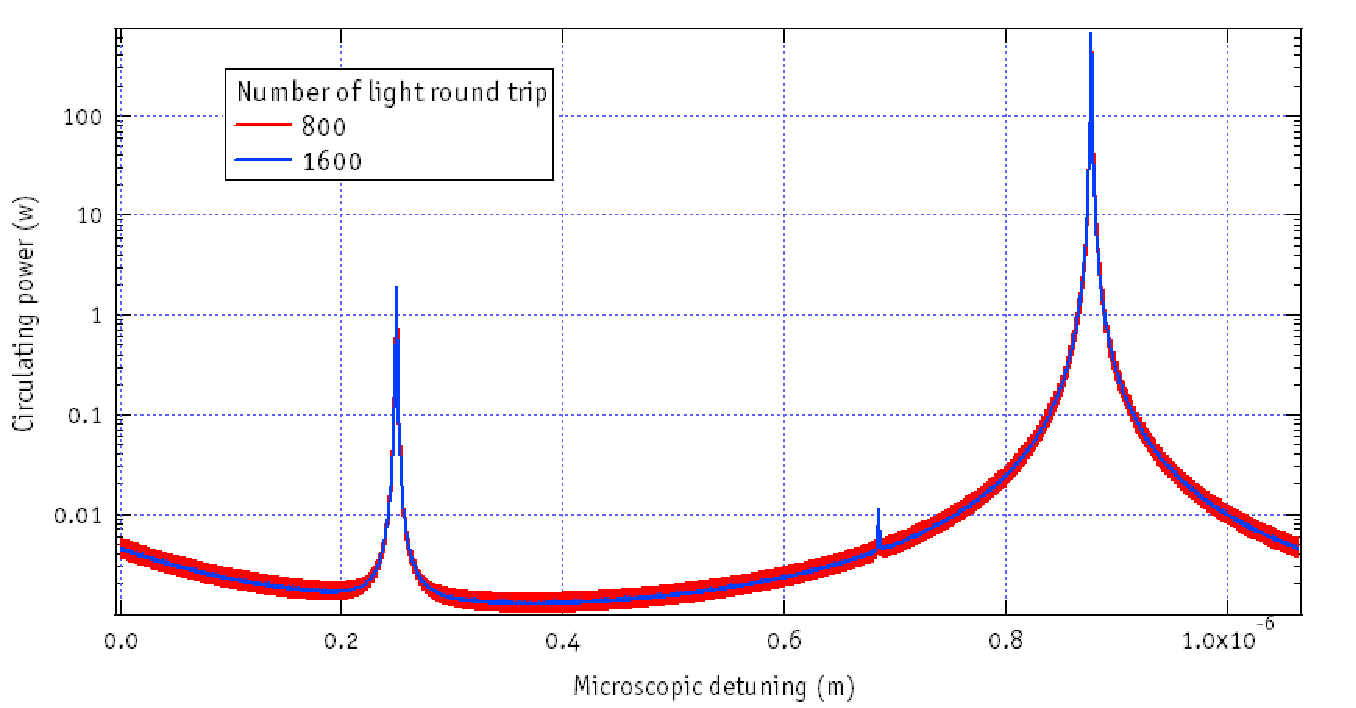
\includegraphics[width = 0.95\textwidth]{Fig2_resonance.pdf}
\end{center}
\caption{\label{fig2:cavres} Circulating power in the cavity as the function of the macroscopic round trip length detuning scanned over one wavelength. The higher peak indicates the resonance position of the fundamental mode TEM$_{00}$. We can also notice two smaller peak revealing the presence of higher order optical modes, this is a strong proof that the input beam is not matched with the cavity eigen mode. The figure has been plotted for two values of \emph{Length.nb\_iter}, this variable determines the number of field $E_i$ to cumulate when calculating the circulating power. On resonance, the build up circulating power is of course higher when we use 1600 fields instead of 800 (even if it is not obvious in the figure due to the large vertical scale).}
\end{figure}



Practically, in OSCAR to draw the plot in figure \ref{fig2:cavres}, a technique first described by Gordon and Li\cite{Gordon} is employed. The principle is explained by the follow step:
\begin{enumerate}
  \item First all the fields $E_i$ are calculated and stored for an arbitrary position of the cavity tuning (so for an arbitrary resonance length). This step is only done once.
  \item The circulating field $E_{circ}$ for a particular microscopic round trip length $\delta l$ is built up by summing all the field $E_i$ with the proper phase shift:
      \begin{equation}
      \label{eq2:buildup}
      E_{circ} = \sum_i E_i \exp\left(j k \delta l \right)
      \end{equation}
  \item Repeat the previous step over all the detuning length $\delta l$ we wish to try.
\end{enumerate}

The advantage of this technique is that the FFT code is just called once to calculate the field $E_i$, then the reconstruction of the power buildup for the various length detuning is just a matter of summing and multiplication. The only limitation of this technique is that a huge amount of memory is required since all the fields $E_i$ are to be stored. For example if we would like to store 500 complex matrices of 256 $\times$ 256 points,  500 megabytes of free memory is required.

%Example iter_propafield

\subsection{Code implementation}
\label{sec2:2.2.3}
To calculate the resonance length in OSCAR, so to calculate the value of \textsl{Length.reso\_zoom}, several script are involved. Here the list:

\begin{itemize}
  \item \textcolor{blue}{Find\_resonance\_length.m} is the main procedure. At the end of the procedure, the variable \textsl{Length.reso\_zoom} which maximises the cavity circulating power, is returned. This script is divided into two similar parts: first part the cavity detuning is scanned over one wavelength, then in the second part we scan around the maximum position found after the first scan with a much greater detuning resolution (we zoom around the maxima found in the first part). At the beginning of the script, two important variables are defined: \emph{Length.nb\_iter} determines the number of step used to scan the cavity over one wavelength (usually 2000) and \emph{Length.nb\_propa\_field} is the number of light round trip taken into account when calculating the circulating power (i.e. number of fields $E_i$ we used).
  \item \textcolor{blue}{Propagate\_Field.m} is script called at the beginning of \textcolor{blue}{Find\_resonance\_length.m}. This script calculates all the intermediate field $E_i$ using the FFT code and stores the results in one variable called \emph{Field.propa}. \emph{Field.propa} is a 3D matrix having with a size of \emph{Grid.Num\_point} $\times$ \emph{Grid.Num\_point} $\times$ \emph{Length.nb\_propa\_field}.
  \item \textcolor{blue}{Build\_Field\_Cavity.m} is a function called intensively by \textcolor{blue}{Find\_resonance\_length.m}. This function takes for argument a length detuning and returns the build-up circulating  field following the equation \ref{eq2:buildup}.
  \item \textcolor{blue}{Calculate\_power.m} is a simple function which takes for input a 2D electric field and returns the optical power in Watt of the input field.
\end{itemize}

\subsection{Some comments}

The method used by OSCAR to find the resonance length is slow. In term of calculation time, it is the bottleneck of this FFT code. It is possible to find different approaches to calculate the resonance length and some are much faster, however I prefer to keep the method described above. Why ? because the plot of the circulating power as a function of the wavelength (figure \ref{fig2:cavres}) contains numerous essential information which help debugging the simulation or understanding the optical system. Here some examples:

\begin{itemize}
  \item If during a simulation, the plot of the circulating power as a function of the detuning does not look like the one in figure \ref{fig2:cavres}, but instead looks flat or with very small bumps it means the cavity is unstable. In the same idea, the linewidth of the peak in the plot is inversely proportional to the finesse of the cavity so it is a good indication of the round trip loss in the cavity.
  \item The number of peaks in the plot is directly proportional to the mode mismatching or misalignment between the input beam and the cavity eigen modes. In the case of perfect mode matching only one peak is present, which means that all the input light coupled to only one optical mode (preferably the fundamental Gaussian beam). By looking at the shape of the higher order modes which are excited (see figure \ref{fig2:cavres}), we could have an idea of the type of mode mismatching and/or misalignment. For example, if all the higher order modes which are excited looks like TEM$_{m0}$, it means the input beam is misaligned with the cavity axis in the horizontal direction.
  \item Finally, since we also know the position detuning for the higher order modes, we can also set the cavity on the resonance of the higher order modes if necessary. The knowledge of the relative detuning position of the resonance for the higher order modes allows also the calculation of the Gouy phase shift between higher order modes (which maybe unknown if the beam is not Gaussian).\\
\end{itemize}

We do not need a lot of light round trip to have an accurate result for the resonance length position. In the previous example, we use 800 or 1600 round trips for the calculation but only 50 round trips can already give a correct answer. The only difference is that the plot of the circulating power as a function of the detuning may not look so sharp (so we can miss the presence of smaller resonance peaks).\\

For verification purpose, it may be important to check the shape of the circulating field for different detuning length. For example to display the circulating field for a detuning position of $2.5 \times 10^{-7}$ which corresponds to the first left peak in the figure \ref{fig2:cavres}, we just have to write the following command in Matlab:

\vspace*{0.5cm}

$>>$ Plot\_Field(Build\_Field\_Cavity(2.5E-7))

\vspace*{0.5cm}
\noindent With such command, we can check which optical modes can build up in the cavity. The 2D amplitude of the three optical modes corresponding to the three peaks in figure \ref{fig2:cavres} are presented in figure \ref{fig2:HOM} in the order of increasing detuning.

% 17 14

\begin{figure}
\begin{center}
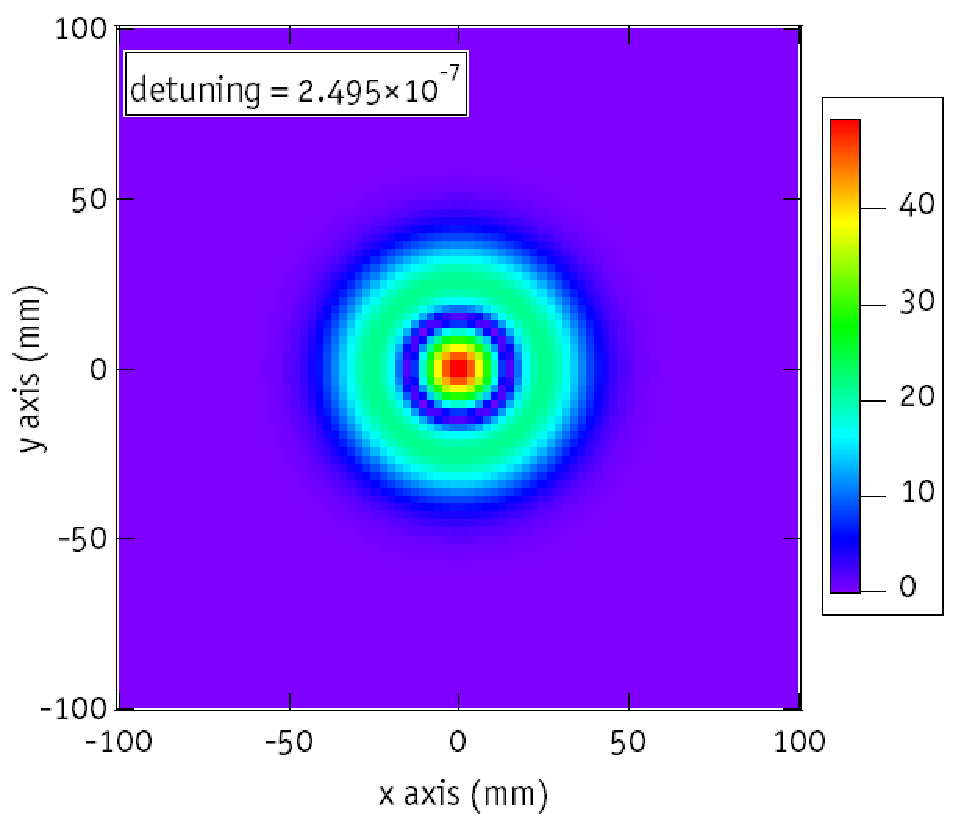
\includegraphics[width = 0.33\textwidth]{Fig2_mode1.pdf}\hfill
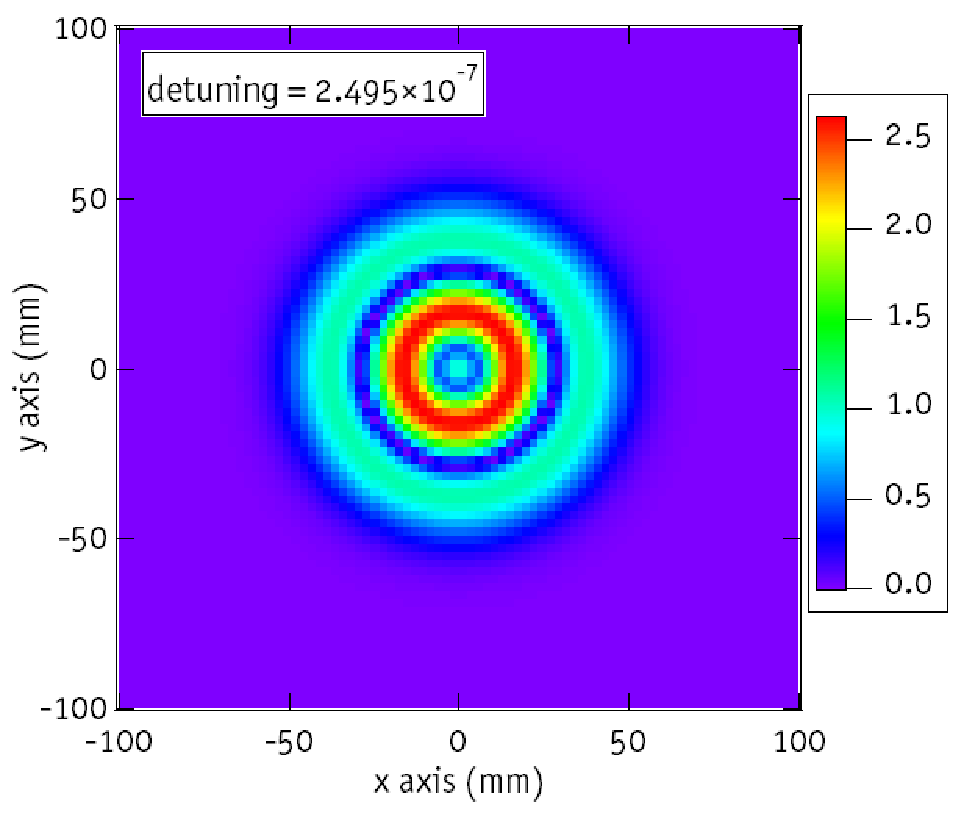
\includegraphics[width = 0.33\textwidth]{Fig2_mode2.pdf}\hfill
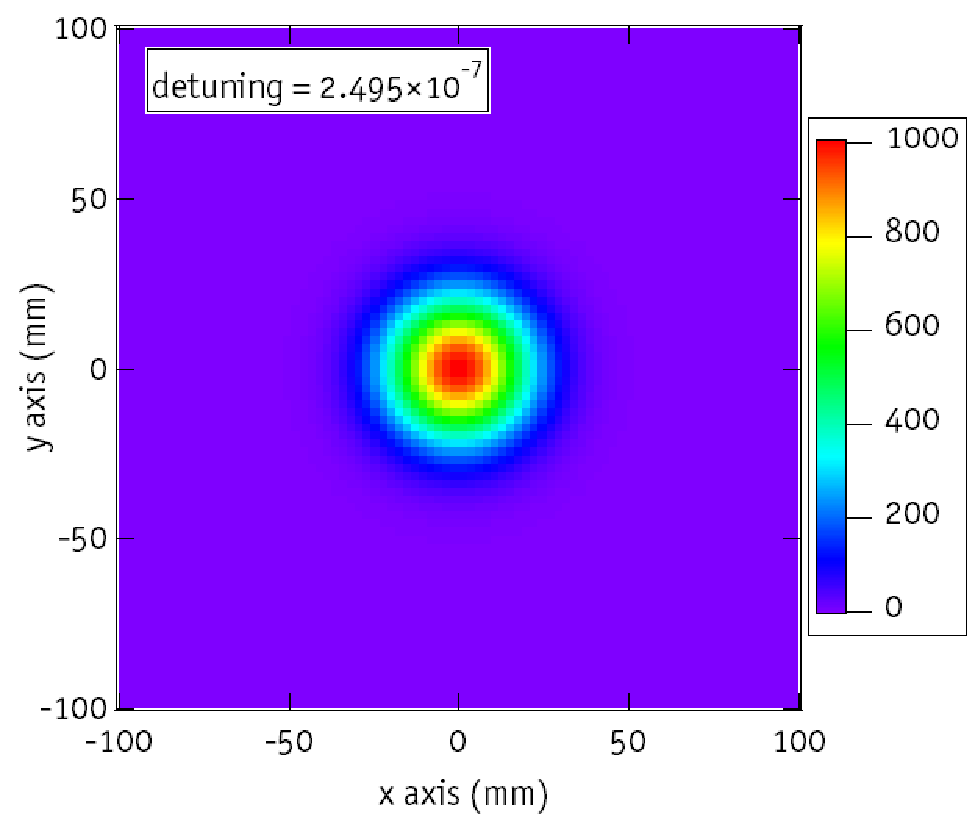
\includegraphics[width = 0.33\textwidth]{Fig2_mode3.pdf}\hfill
\end{center}
\caption{\label{fig2:HOM} 2D amplitude of the circulating field responsible for the 3 peaks in the plot of the cavity circulating as a function of the detuning (figure \ref{fig2:cavres}). We can recognise from left to right the mode LG$_{10}$, LG$_{20}$ and finally the fundamental mode LG$_{00}$. The presence of the there first LG$_{m0}$ optical modes indicates that the input beam is properly aligned with the cavity axis but we have a slight mode mismatching. }
\end{figure}

\section{Calculating the circulating field}
\label{sec2:4}
The previous procedure \textcolor{blue}{Find\_resonance\_length.m} is essential to determine the operating point for the cavity. In most cases the cavity is locked on the fundamental mode TEM$_{00}$, so the procedure \textcolor{blue}{Find\_resonance\_length.m} returns by default the value of the detuning required to make the TEM$_{00}$ resonant inside the cavity. It is always implicitly assumed that the maximum circulating power is obtained for a resonant TEM$_{00}$ and not for a higher order optical mode.\\

After we have calculated the resonance length, the script \textcolor{blue}{Get\_results.m} can be called. This script calculates the static fields in the Fabry perot cavity and displayed the total circulating power as well as other results.\\

The procedure to calculate the circulating field was explained in the section \ref{sec1.4} and is briefly reminded here. First the input laser field (variable \emph{Field.Start} in OSCAR) crosses the input test mass substrate, creating the intermediate circulating field (variable \emph{Field.Circ} and also called $E_1$ in figure \ref{fig1:cavity}). Then the intermediate circulating field is propagated back and forth between the cavity mirrors with the number of round trip determined by the variable \emph{Iter.final}. The total circulating field (variable \emph{Field.Total}) is derived by summing all the field intermediate field at a defined position in the cavity, in OSCAR it is done after the reflection from the input mirror. Everything described above can be simply achieved in Matlab as shown in the listing \ref{lis2:cav_circ}.\\

\begin{lstlisting}[float=htp,caption=The core of the OSCAR programm to calculate the circulating field in a cavity\label{lis2:cav_circ},frame=lines]

Length.reso_zoom = 8.7794200e-007;
Iter.final = 3000;

Phase_shift =  exp(i*Laser.k_prop* Length.reso_zoom);

Field.Circ = Propa_mirror(Field.Start, Mirror.ITM_trans,i*ITM.t);

for q = 1:Iter.final

    Field.Total = Field.Total + Field.Circ;

    Field.Circ = Make_propagation(Field.Circ,Mat_propagation);
    Field.Circ = Propa_mirror(Field.Circ,Mirror.ITM_cav,ETM.r);
    Field.Circ = Make_propagation(Field.Circ,Mat_propagation);
    Field.Circ = Field.Circ * Phase_shift;
    Field.Circ = Propa_mirror(Field.Circ, Mirror.ITM_cav,ITM.r);

end

\end{lstlisting}

After the calculation of the total circulating field in the cavity \emph{Field.Total}, the transmitted beam \emph{Field.Transmit} and the reflected beam \emph{Field.Reflect} can be easily derived. The transmitted beam is simply the total circulating field after a transmission through the end mirror. The reflected beam is the sum of the input field directly reflected by the input mirror and the field leaking from the cavity (which is the total circulating field transmitted by the input mirror).\\

\section{Displaying the results}
\label{sec2:5}
After the total circulating field, the transmitted field and the reflected field have been calculated, the results can be displayed. First some parameters (with obvious names) are written in the Matlab command window, then a 2D plot of the different optical fields present is displayed as shown in figure \ref{fig2:display}.

\begin{verbatim}
 ------ Display the results ------
 Circulating power (W): 749.256602
 Reflected power (W): 0.885891
 Transmitted power (W): 0.037463
 Beam radius on the ITM (m): 0.020574
 Beam radius on the ETM (m): 0.020577
 Cavity waist size (m): 0.016462
 Location of the waist from ITM (m): -499.853070
\end{verbatim}

\begin{figure}
\begin{center}
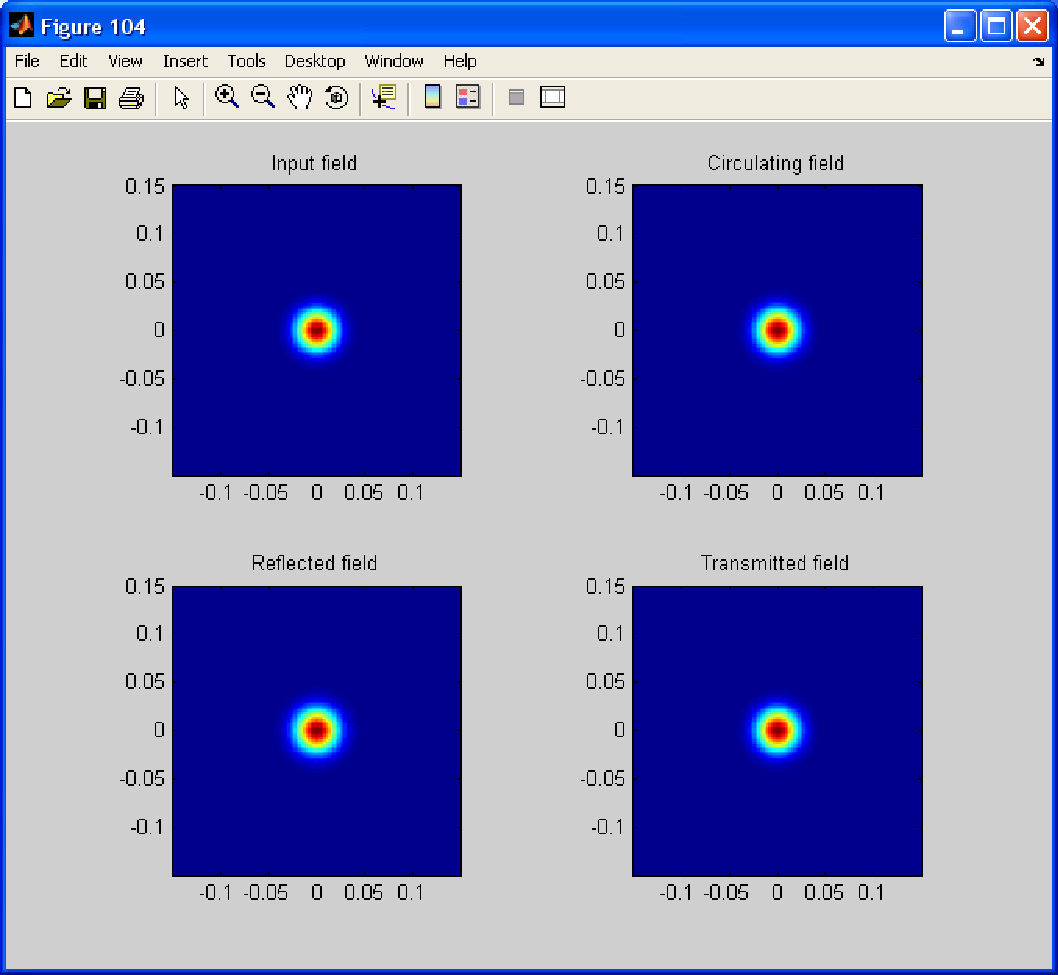
\includegraphics[width = 0.75\textwidth]{Fig2_results.pdf}
\end{center}
\caption{\label{fig2:display} Amplitude profile of the different steady state optical fields in the Fabry Perot cavity. }
\end{figure}

To feel confident in the results from OSCAR, it is always good to test the results with different parameters for the number of light round trip or the size of the grid. If the results are very sensitive to one parameters, it usually means that there is a problem somewhere, and further checks are required.

For example, the results as a function of number of light round trip are presented in the table \ref{tab2:RT}. As expected on resonance, the circulating power, defined by the power of the sum of all the fields $E_i$ increases when the number of field $E_i$ computed increases. The right number of iteration to consider for a simulation depends on the finesse of the cavity. For a low finesse cavity, with a high round trip loss, the power contained in the field $E_i$ will quickly decrease and rapidly becomes negligible after few round trips. In table \ref{tab2:RT}, the FFT results are compared with the results from the software Finesse \cite{Finesse}, which is based on mode expansion. The Finesse script used to simulate the Fabry Perot cavity is presented in appendix \ref{chaB}.\\

\begin{table}[tbp]
  \centering
  \caption{\label{tab2:RT} Influence of the total number of light round trip considered (variable \emph{Iter.final}) on the results. The size of the grid is set to 128 $\times$ 128.}
\begin{tabular}{|l|c|c|c|}
\hline
Number of  & Circulating & Cavity waist & Cavity waist \\
iteration &  power (W) & size (mm) &  position from IM (m) \\
\hline
1000 &  640.712 &  18.403 & -499.835 \\
2500 &  747.546 &  18.403 & -499.852 \\
5000 &  749.903 &  18.403 & -499.853 \\
10000 &  749.906 &  18.403 & -499.835 \\
\hline
\hline
Finesse &  749.906 &  18.403 & -500 \\
\hline
\end{tabular}
\end{table}

Another important parameter to test is the resolution of the grid. The results for different sizes of the grid are presented in the table \ref{tab2:grid_size}. As we can see the results are pretty robust even with a coarse grid. For a grid size of 32 $\times$ 32, the grid resolution is 1~cm, which means the beam radius is just represented by 2 pixels in the cavity. Even with such a low resolution, the results are still accurate.

\begin{table}[tbp]
  \centering
  \caption{\label{tab2:grid_size} Influence of the size of the grid (variable \emph{Grid.Num\_point}) on the results. The number of iteration is 5000. The computation time is normalised by the computation time required for a grid of size 128 $\times$ 128 (which is less than 2 minutes on a modern computer).}
\begin{tabular}{|l|c|c|c|c|}
\hline
Size of   & Circulating & Cavity waist & Cavity waist & Normalised \\
the grid &  power (W) & size (mm) &  position from IM (m) & computation time\\
\hline
32 $\times$ 32 &  749.902 &  18.403 & -499.854 & 0.09 \\
64 $\times$ 64 &  749.903 &  18.403 & -499.853 & 0.31 \\
128 $\times$ 128 &  749.903 &  18.403 & -499.853 & 1.00 \\
256 $\times$ 256 &  749.902 & 18.403 & -499.844 & 7.32\\
\hline
\hline
Finesse &  749.906 &  18.403 & -500 & - \\
\hline
\end{tabular}
\end{table}


%Circulating field
%
%?Other field
%
%
%
%More points
%
%comparison finesse result, size of the grid, finesse
%
%equivalent finesse file in annexe

%128 * 128
% Nb iter     Pcirc      Pref       Beam size ITM Cavity waist    Waist position
% 1000
% 2500
% 5000
% 10000
%
%10000
%Circulating power (W): 749.906250
% Reflected power (W): 0.887468
% Transmitted power (W): 0.037495
% Beam radius on the ITM (m): 0.020574
% Beam radius on the ETM (m): 0.020577
% Cavity waist size (m): 0.018403
% Location of the waist from ITM (m): -499.853070
%
% 5000
%  Circulating power (W): 749.902530
% Reflected power (W): 0.887459
% Transmitted power (W): 0.037495
% Beam radius on the ITM (m): 0.020574
% Beam radius on the ETM (m): 0.020577
% Cavity waist size (m): 0.018403
% Location of the waist from ITM (m): -499.853070
%
% 2500
%
%  Circulating power (W): 747.545912
% Reflected power (W): 0.881741
% Transmitted power (W): 0.037377
% Beam radius on the ITM (m): 0.020574
% Beam radius on the ETM (m): 0.020577
% Cavity waist size (m): 0.018403
% Location of the waist from ITM (m): -499.852995
%
% 1000
% Circulating power (W): 640.712171
% Reflected power (W): 0.633378
% Transmitted power (W): 0.032036
% Beam radius on the ITM (m): 0.020574
% Beam radius on the ETM (m): 0.020577
% Cavity waist size (m): 0.018403
% Location of the waist from ITM (m): -499.835107
%
% 5000 iter
%
% 64*64
% Circulating power (W): 749.902653
% Reflected power (W): 0.887459
% Transmitted power (W): 0.037495
% Beam radius on the ITM (m): 0.020574
% Beam radius on the ETM (m): 0.020577
% Cavity waist size (m): 0.018403
% Location of the waist from ITM (m): -499.853236
%Elapsed time is 34.988457 seconds.
%
%32*32
% Circulating power (W): 749.902499
% Reflected power (W): 0.887459
% Transmitted power (W): 0.037495
% Beam radius on the ITM (m): 0.020574
% Beam radius on the ETM (m): 0.020577
% Cavity waist size (m): 0.018403
% Location of the waist from ITM (m): -499.854544
%Elapsed time is 10.540556 seconds.
%
%128*128
% Circulating power (W): 749.902530
% Reflected power (W): 0.887459
% Transmitted power (W): 0.037495
% Beam radius on the ITM (m): 0.020574
% Beam radius on the ETM (m): 0.020577
% Cavity waist size (m): 0.018403
% Location of the waist from ITM (m): -499.853070
%Elapsed time is 111.589948 seconds.
%
%256*256
%Circulating power (W): 749.902387
% Reflected power (W): 0.887459
% Transmitted power (W): 0.037495
% Beam radius on the ITM (m): 0.020574
% Beam radius on the ETM (m): 0.020577
% Cavity waist size (m): 0.018403
% Location of the waist from ITM (m): -499.844147
%Elapsed time is 817.170512 seconds.

\section{Calculating the cavity eigen-mode and diffraction loss}
\label{sec2:6}
We can first wonder what is called a cavity eigen-mode ? A cavity eigen mode is an electric field which comes back exactly with the same spatial profile after one cavity round trip. The spatial profile must be identical but not necessary the amplitude since the cavity may be lossy. The usual cavity eigen modes are the set of Hermitte-Gauss and Laguere-Gauss for cavity with spherical mirrors, as most of the readers must already know.

For high finesse cavity\footnote{Quantitatively (and approximatively), we could say that a cavity has a high finesse when the the circulating power is much higher than the input power}, the circulating field is in fact a cavity eigen mode. This can be easily understood if the input cavity field is negligible in front of the cavity circulating field, a more rigorous demonstration can be found in \cite{Saha:97} for example. Mode cleaner cavities are based on this principle, the transmitted beam is the TEM$_{00}$ cavity eigen-mode, whereas the input beam may be composed of several optical modes.

Usually, we seldom need a FFT code to calculate the eigen modes of a Fabry Perot cavity with spherical mirrors since the exact analytical solutions are known \cite{Koechner}. However, we may want to know the cavity eigen modes if the mirrors are not perfectly spherical (because of thermal lensing) or if beam clipping due to finite size mirrors is important. To know the cavity eigen modes in this case, we defined an input beam close in shape to the supposed cavity eigen modes and then calculate the cavity circulating field. The cavity circulating field will be the cavity eigen mode. Some problems may arise if the cavity is nearly degenerated and the input beam is composed of several resonant or near resonant modes. In this case we can think of two solutions:
\begin{enumerate}
  \item Increase the cavity finesse to have a better separation between optical modes and if necessary generate some specific losses to attenuate the undesirable optical modes.
  \item Take the cavity circulating field as a new input field and start a new calculation. This step can be done several times and could be understood as cascading optical cavities to increase the mode cleaning effect.
\end{enumerate}

Since we have now an idea about how to calculate a cavity eigen mode, we can also try to calculate the diffraction loss for this mode. We called diffraction loss, the loss due to the finite size of the mirrors. This loss is also sometime referred as clipping loss. Since in theory, Gaussian beams have an infinite spatial extend, diffraction losses are always present. However the loss can become negligible for large diameter mirrors and
small laser beam radius. For example, the diffraction loss of a laser beam of beam radius 6~cm after reflection on a 15~cm radius mirror is only 4~ppm \cite{Siegman}. The diffraction loss are more important for higher order optical modes and ultimately can even affect the profile of the mode \cite{Pab}.\\

In OSCAR the diffraction loss of an eigen mode is computed by calculating the round trip loss of the mode when the reflectivities of the cavity mirrors are set to 1. So the first step is to calculate the cavity eigen mode, this is usually done by calculating the circulating field in a high finesse cavity. The second step is to normalised the power of the eigen mode to 1 and then propagate the mode one round trip in the cavity whose mirrors reflectivities are set to 1. Finally, the diffraction loss is simply the power lost by the mode during one round trip. The above steps are shown in the listing \ref{lis2:diffloss}.

\begin{lstlisting}[float=tp,caption=Piece of code used to calculate the diffraction loss. We suppose that we have already calculate the circulating field \emph{Field.Total}. \label{lis2:diffloss},frame=lines]
% Normalise the circulating field (=the eigen-nmode)
Field.loss = Field.Total;
Field.loss = Field.loss/sqrt(Calculate_power(Field.loss));

% Make a round trip with a reflectivity of 1 for the mirrors
Field.loss = Make_propagation(Field.loss,Mat_propagation);
Field.loss = Propa_mirror(Field.loss,Mirror.ETM_cav,1);
Field.loss = Make_propagation(Field.loss,Mat_propagation);
Field.loss = Propa_mirror(Field.loss, Mirror.ITM_cav,1);

% Calculate the diffraction loss
Dif_loss = (1 - Calculate_power(Field.loss));
fprintf('Diffraction loss per round trip: %d \n',Dif_loss);
\end{lstlisting}

An example about how to calculate diffraction loss with OSCAR can be found in the folder called \textcolor{blue}{Calculate\_diffraction\_loss}. This example is detailed in the chapter \ref{cha3.2} of this manual.

\section{A typical OSCAR run}

A typical run of OSCAR consists of running consecutively three different Matlab scripts:

\begin{enumerate}
  \item \textcolor{blue}{CreateField.m}, is the script used to initialised the variables and defined the optical cavity parameters, the mirror maps as well as the input beam.
  \item \textcolor{blue}{Find\_resonance\_length.m} is used to find automatically the resonance length of the cavity which maximise the circulating power. In most cases, the resonance length locks the cavity on the TEM$_{00}$. Manually it is possible to lock the cavity on any arbitrary position, for example to see the resonance of one higher order mode.
  \item \textcolor{blue}{Get\_results.m} is the main procedure which get the circulating field in the cavity and if required also the reflected and transmitted fields and the diffraction loss of the circulating field.
\end{enumerate}

The call for three previous script are usually reunited into one single scrip called \textcolor{blue}{Run\_OSCAR.m}.

\section{Script and function list}

Here the list of Matlab scripts that you may find in every OSCAR folders. Depending on the goal of the simulation, the scripts may not be exactly the same and some variations exist.

\begin{itemize}
  \item \textcolor{blue}{Beam\_parameter.m}, a function which takes for parameter a complex 2D Gaussian field and returns the beam radius and the wavefront radius of curvature. The fit only works for fundamental Gaussian beam but it can easily be adapted to also fit higher order modes.
  \item \textcolor{blue}{Build\_Field\_Cavity.m} is a function used to find the resonance length, see section \ref{sec2:2.2.3}.
  \item \textcolor{blue}{Calculate\_power.m} a simple function which takes a 2D field and returns the optical power of the field.
  \item \textcolor{blue}{CreateField.m}, the first script called in OSCAR to initialise all the variables, see section \ref{sec2:2.2}.
  \item \textcolor{blue}{CreateMirror.m} script to create the matrix representing the wavefront distortion induced by the mirrors, see section \ref{sec1:3:2}.
  \item \textcolor{blue}{Find\_resonance\_length.m} script to find the microscopic detuning required to set the cavity on resonance, see section \ref{sec2:3}.
%  \item \textcolor{blue}{Fit\_Gaussian.m} small function called by \textcolor{blue}{Beam\_parameter.m}. As the name says, the function does a 1D fit of a Gaussian beam at the waist.
  \item \textcolor{blue}{Get\_results.m} main OSCAR procedure to calculate the circulating power in the cavity. The script is also used to do some post processing of the results, see section \ref{sec2:4} and \ref{sec2:5}.
  \item \textcolor{blue}{Make\_propagation.m} propagates a 2D field over a certain distance. The function takes two arguments a field and a propagation matrix and return the field after propagation. The function is the implementation of the last three lines in listing \ref{lis1:start2}.
  \item \textcolor{blue}{Plot\_Field.m}, a function which takes a 2D field and plots the amplitude of the field in 2D (or 3D if it is desired).
  \item \textcolor{blue}{Propa\_mirror.m} a function to simulate the effect of a wavefront distortion. The function takes a 2D input field, a mirror map or any distortion and a reflectivity (or transmission) and returns the field after reflection (or transmission). The function is described in section \ref{sec1:3:5}.
  \item \textcolor{blue}{Propagate\_Field.m} creates the initial 3D matrix used to calculate the circulating field for the different detuning, see section \ref{sec2:2.2.3} for further explanations.
\end{itemize}



